%-----------------------------------------------------------------
%	BOOTSTRAP: TESTING THE ASSUMPTIONS
%	!TEX root = ./../main.tex
%-----------------------------------------------------------------
\subsection{Testing the linear regression assumptions}\label{ssec:testing-assumptions}
As stated in \Cref{sec:simple-regression}, in linear regression the standard errors and hypothesis tests associated with the linear model rely on the random error $\epsilon$ being normal, independent, and homoscedastic.

Therefore, to be sure the results found on \Cref{sec:reg-analysis-data} are reliable, we should test these assumptions using the regression diagnostic tools introduced in \Cref{sec:reg-analysis-issues}. First we will analyse the North Atlantic basin data, and then we will analyse the Northeast Pacific basin data.

\bigskip
The first step is to have a look at the diagnostic plots. The diagnostic plots for the North Atlantic basin, separating the data by SST class can be observed in \Cref{fig:natl_residuals}.
\begin{figure}[H]
	\centering
	\subfloat[Q-Q plot (low SST)]{%
		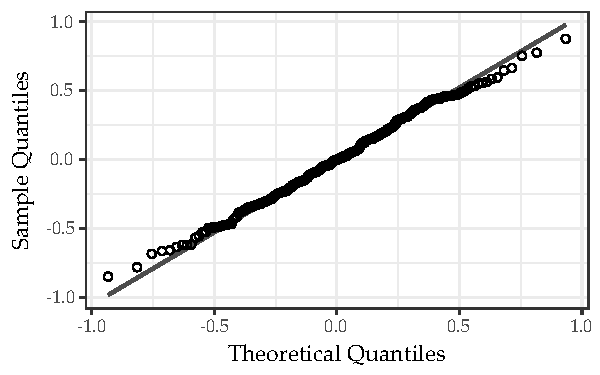
\includegraphics[width=0.45\textwidth]{./images/natl_low_resid_qqplot}
		\label{fig:natl_low_resid_qqplot}%
		}%
	\subfloat[Residuals vs fitted (low SST)]{%
		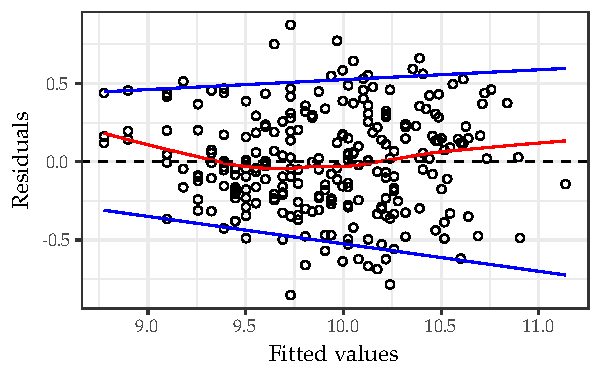
\includegraphics[width=0.45\textwidth]{./images/natl_low_resid_fitted}
		\label{fig:natl_low_resid_fitted}%
		}%
	\\
	\subfloat[Q-Q plot (high SST)]{%
		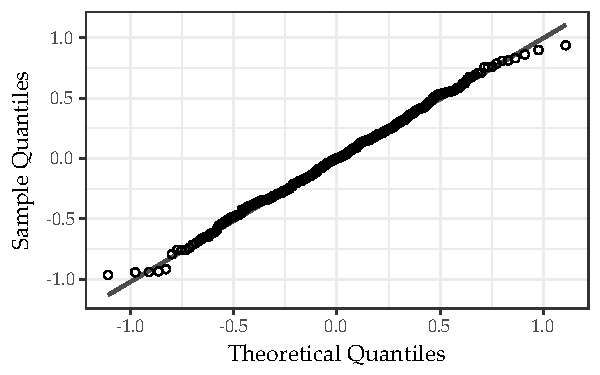
\includegraphics[width=0.45\textwidth]{./images/natl_high_resid_qqplot}
		\label{fig:natl_high_resid_qqplot}%
		}%
	\subfloat[Residuals vs fitted (high SST)]{%
		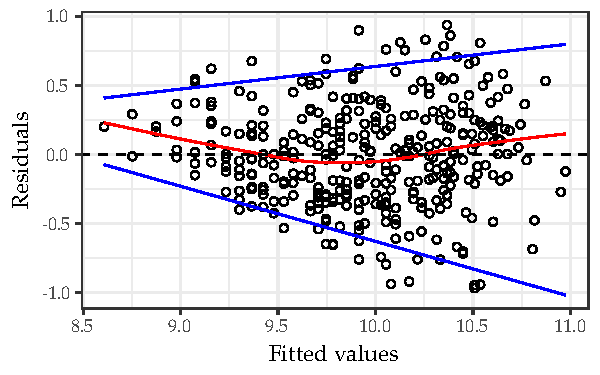
\includegraphics[width=0.45\textwidth]{./images/natl_high_resid_fitted}
		\label{fig:natl_high_resid_fitted}%
		}%
	\caption{Diagnostic plots to analyse the residuals for the North Atlantic basin}
	\label{fig:natl_residuals}
\end{figure}
In the Q-Q plots shown in \Cref{fig:natl_low_resid_qqplot} and \Cref{fig:natl_high_resid_qqplot} we can see that the residuals are mostly normal; if anything, the distribution has light tails. The residual plots in \Cref{fig:natl_low_resid_fitted} and \Cref{fig:natl_high_resid_fitted}, however, tell show us gross heteroscedasticity, specially for high-SST years.

To confirm this numerically, let us explore the results of performing the Lilliefors, correlation, and Breusch--Pagan tests for the North Atlantic basin in \Cref{tab:stat-tests-natl}.
\begin{table}[H]
	\centering
	\begin{tabular}{lccc}
		\toprule
		\toprule
		Data     & Lilliefors   & Correlation  & Breusch--Pagan \\
		\midrule
		Low-SST  & \num{0.7416} & \num{1.0000} & \num{0.0376}   \\
		High-SST & \num{0.9740} & \num{1.0000} & \num{0.0002}   \\
		\bottomrule
	\end{tabular}
	\caption{List of $p$-values associated with the statistical hypothesis tests to respectively analyse normality, independence, and homoscedasticity of the residuals on the low-SST and high-SST subsets of the North Atlantic basin}
	\label{tab:stat-tests-natl}
\end{table}
The $p$-values tell us that the only rejected hypothesis is homoscedasticity for both datasets, which is precisely what we observed on the residual plots.

\bigskip
For the Northeast Pacific basin we see a similar picture. The diagnostic plots for the this basin, separating the data by SST class can be observed in \Cref{fig:epac_residuals}.
\begin{figure}[H]
	\centering
	\subfloat[Q-Q plot (low SST)]{%
		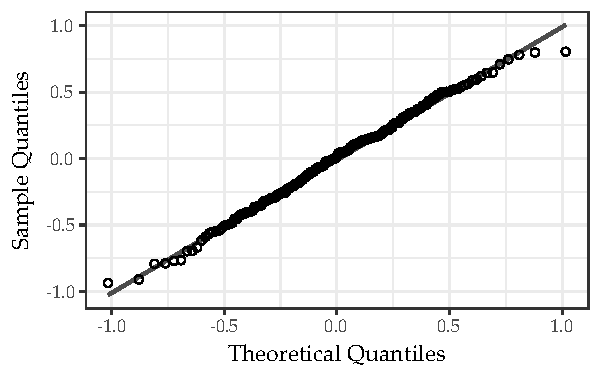
\includegraphics[width=0.45\textwidth]{./images/epac_low_resid_qqplot}
		\label{fig:epac_low_resid_qqplot}%
		}%
	\subfloat[Residuals vs fitted (low SST)]{%
		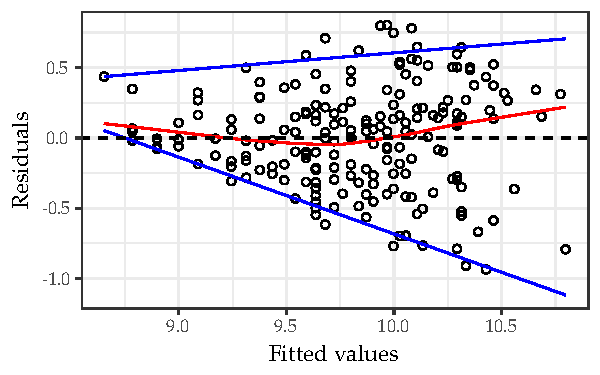
\includegraphics[width=0.45\textwidth]{./images/epac_low_resid_fitted}
		\label{fig:epac_low_resid_fitted}%
		}%
	\\
	\subfloat[Q-Q plot (high SST)]{%
		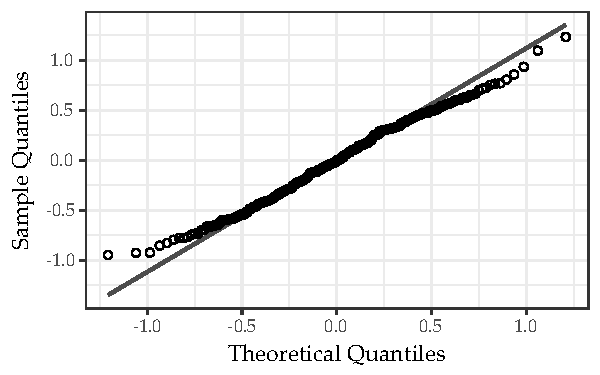
\includegraphics[width=0.45\textwidth]{./images/epac_high_resid_qqplot}
		\label{fig:epac_high_resid_qqplot}%
		}%
	\subfloat[Residuals vs fitted (high SST)]{%
		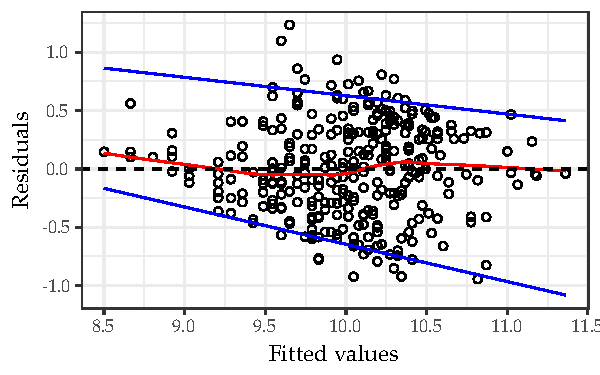
\includegraphics[width=0.45\textwidth]{./images/epac_high_resid_fitted}
		\label{fig:epac_high_resid_fitted}%
		}%
	\caption{Diagnostic plots to analyse the residuals for the Northeast Pacific basin}
	\label{fig:epac_residuals}
\end{figure}
In the Q-Q plot shown in \Cref{fig:epac_low_resid_qqplot} we can see that the residuals for low-SST year follow a normal distribution with light tails. The Q-Q plot for high-SST years shown in \Cref{fig:epac_high_resid_qqplot}, however, is strongly non-normal. The residual plots in \Cref{fig:epac_low_resid_fitted} and \Cref{fig:epac_high_resid_fitted} tell show us quite heteroscedastic residuals, specially for low-SST years.

Again, to confirm this numerically, we explore the results of performing the Lilliefors, correlation, and Breusch--Pagan tests for the Northeast Pacific basin seen in \Cref{tab:stat-tests-epac}.
\begin{table}[H]
	\centering
	\begin{tabular}{lccc}
		\toprule
		\toprule
		Data     & Lilliefors   & Correlation  & Breusch--Pagan \\
		\midrule
		Low-SST  & \num{0.7106} & \num{1.0000} & \num{0.0000}   \\
		High-SST & \num{0.0217} & \num{1.0000} & \num{0.1974}   \\
		\bottomrule
	\end{tabular}
	\caption{List of $p$-values associated with the statistical hypothesis tests to respectively analyse normality, independence, and homoscedasticity of the residuals on the low-SST and high-SST subsets of the Northeast Pacific basin}
	\label{tab:stat-tests-epac}
\end{table}
In this case, for low-SST years the rejected hypothesis is homoscedasticity, while for the high-SST years normality is the rejected hypothesis. This is precisely what we observed on the residual plots.

\bigskip
Having heteroscedasticity and non-normality tells us we cannot fully rely on the calculated standard errors, and we need to use bootstrap to obtain a more robust linear model to be able to infer statistical properties of the data using linear regression as the underlying model.
